\documentclass[aspectratio=169]{beamer}

% ─── Theme ───────────────────────────────────────────────────────────────────
\usetheme{Madrid}
\setbeamertemplate{navigation symbols}{}
\setbeamertemplate{footline}[frame number]

% ─── Packages ────────────────────────────────────────────────────────────────
\usepackage[utf8]{inputenc}
\usepackage[T1]{fontenc}
\usepackage{lmodern}
\usepackage{listings}
\usepackage{xcolor}
\usepackage{tikz}
\usepackage{booktabs}
\usepackage{array}
\usepackage{amsmath}
\usepackage{pifont}

\usetikzlibrary{arrows.meta, shapes.geometric, positioning, fit, backgrounds, calc, decorations.pathreplacing}

% ─── Colours ─────────────────────────────────────────────────────────────────
\definecolor{primary}{HTML}{1A3A5C}
\definecolor{accent}{HTML}{2980B9}
\definecolor{colgreen}{HTML}{27AE60}
\definecolor{colorange}{HTML}{E67E22}
\definecolor{colred}{HTML}{C0392B}
\definecolor{codebg}{HTML}{F0F4F8}
\definecolor{kw}{HTML}{0033B3}
\definecolor{str}{HTML}{067D17}
\definecolor{cmt}{HTML}{8C8C8C}
\definecolor{lightblue}{HTML}{EBF5FB}
\definecolor{lightgray}{HTML}{F5F5F5}
\definecolor{stagecol1}{HTML}{D6EAF8}
\definecolor{stagecol2}{HTML}{D5F5E3}
\definecolor{stagecol3}{HTML}{FCF3CF}
\definecolor{stagecol4}{HTML}{FDEDEC}
\definecolor{stagecol5}{HTML}{E8DAEF}
\definecolor{stagecol6}{HTML}{E8F8F5}

% ─── Beamer colours ──────────────────────────────────────────────────────────
\setbeamercolor{palette primary}{bg=primary, fg=white}
\setbeamercolor{palette secondary}{bg=accent, fg=white}
\setbeamercolor{palette tertiary}{bg=primary!80, fg=white}
\setbeamercolor{palette quaternary}{bg=primary, fg=white}
\setbeamercolor{structure}{fg=primary}
\setbeamercolor{section in toc}{fg=primary}
\setbeamercolor{alerted text}{fg=colred}
\setbeamercolor{block title}{bg=primary, fg=white}
\setbeamercolor{block body}{bg=lightblue}
\setbeamercolor{block title alerted}{bg=colred, fg=white}
\setbeamercolor{block body alerted}{bg=colred!10}
\setbeamercolor{block title example}{bg=colgreen, fg=white}
\setbeamercolor{block body example}{bg=colgreen!10}

% ─── Code style ──────────────────────────────────────────────────────────────
\lstdefinestyle{py}{
    language=Python,
    backgroundcolor=\color{codebg},
    basicstyle=\ttfamily\scriptsize,
    keywordstyle=\color{kw}\bfseries,
    stringstyle=\color{str},
    commentstyle=\color{cmt}\itshape,
    showstringspaces=false,
    breaklines=true,
    frame=single,
    framerule=0.3pt,
    rulecolor=\color{accent!40},
    xleftmargin=0.5em,
    framexleftmargin=0.5em,
    tabsize=4,
    morekeywords={True, False, None, yield, async, await, with, as},
}
\lstset{style=py}

% ─── Custom commands ─────────────────────────────────────────────────────────
\newcommand{\ic}[1]{\texttt{\small #1}}
\newcommand{\arw}{$\rightarrow$\ }
\newcommand{\done}{\textcolor{colgreen}{\ding{51}}}
\newcommand{\partdone}{\textcolor{colorange}{$\sim$}}
\newcommand{\pending}{\textcolor{colred}{\ding{55}}}

% TikZ styles used throughout
\tikzset{
  pbox/.style={draw=primary, fill=lightblue, rounded corners=4pt, thick,
               text width=#1, align=center, minimum height=0.6cm,
               font=\scriptsize},
  gbox/.style={draw=colgreen, fill=colgreen!10, rounded corners=4pt, thick,
               text width=#1, align=center, minimum height=0.6cm,
               font=\scriptsize},
  obox/.style={draw=colorange, fill=colorange!10, rounded corners=4pt, thick,
               text width=#1, align=center, minimum height=0.6cm,
               font=\scriptsize},
  rbox/.style={draw=colred, fill=colred!10, rounded corners=4pt, thick,
               text width=#1, align=center, minimum height=0.6cm,
               font=\scriptsize},
  abox/.style={draw=accent, fill=accent!10, rounded corners=4pt, thick,
               text width=#1, align=center, minimum height=0.6cm,
               font=\scriptsize},
  stagebox/.style={draw=primary, fill=#1, rounded corners=5pt, thick,
                   text width=2.1cm, align=center, minimum height=1.4cm,
                   font=\scriptsize},
}

% ─── Title ───────────────────────────────────────────────────────────────────
\title[CollectiveOS]{\textbf{CollectiveOS}\\Personal AI Assistant}
\subtitle{Engineering Architecture \& Demo}
\author{Anurag Dhiman}
\date{}

% =============================================================================
\begin{document}
% =============================================================================

% ─── Title slide ─────────────────────────────────────────────────────────────
\begin{frame}
\titlepage
\begin{center}
\small
\textbf{Stack:}\ Python\ $|$\ Google Gemini (function calling)\ $|$\ PostgreSQL + pgvector\\
FastAPI + SSE\ $|$\ VoiceOS (LiveKit + Gemini Live)\ $|$\ APScheduler\ $|$\ structlog
\end{center}
\end{frame}

% ─── Outline ─────────────────────────────────────────────────────────────────
\begin{frame}{Outline}
\tableofcontents
\end{frame}

% =============================================================================
\section{Architecture Overview}
% =============================================================================

\begin{frame}{Architecture Overview}
% ── Top: Problem → System → Components → Data Flow ──────────────────────────
\begin{center}
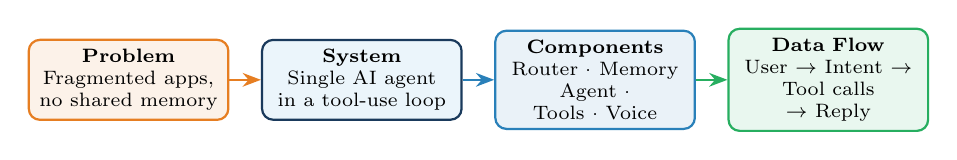
\begin{tikzpicture}[node distance=0.5cm, every node/.style={font=\scriptsize}]
  \node[obox=2.3cm] (prob) {\textbf{Problem}\\Fragmented apps,\\no shared memory};
  \node[pbox=2.3cm, right=0.4cm of prob] (sys) {\textbf{System}\\Single AI agent\\in a tool-use loop};
  \node[abox=2.3cm, right=0.4cm of sys] (comp) {\textbf{Components}\\Router · Memory\\Agent · Tools · Voice};
  \node[gbox=2.3cm, right=0.4cm of comp] (flow) {\textbf{Data Flow}\\User \arw Intent \arw\\Tool calls \arw Reply};
  \draw[-{Stealth}, thick, colorange] (prob) -- (sys);
  \draw[-{Stealth}, thick, accent]    (sys)  -- (comp);
  \draw[-{Stealth}, thick, colgreen]  (comp) -- (flow);
\end{tikzpicture}
\end{center}

\vspace{0.3em}
\begin{columns}[T]
% ── Tech Stack ───────────────────────────────────────────────────────────────
\begin{column}{0.38\textwidth}
\begin{block}{Tech Stack}
\scriptsize
\begin{tabular}{ll}
\textbf{Language}  & Python 3.12 \\
\textbf{LLM}       & Gemini Flash (function calling) \\
\textbf{Voice LLM} & Gemini Live (audio I/O) \\
\textbf{API layer} & FastAPI + SSE \\
\textbf{DB}        & PostgreSQL + pgvector \\
\textbf{Embeddings}& all-MiniLM-L6-v2 \\
\textbf{Scheduler} & APScheduler \\
\textbf{Logging}   & structlog (JSON) \\
\end{tabular}
\end{block}
\end{column}
% ── Key Decisions + Security ──────────────────────────────────────────────────
\begin{column}{0.30\textwidth}
\begin{block}{Key Design Decisions}
\scriptsize
\begin{itemize}
  \item No agent framework — raw Python loop
  \item Two-model cascade: Flash router\\narrows 57 tools before main call
  \item Single Postgres for structured\\data \textit{and} vector search
  \item Daemon threads for async enrichment
\end{itemize}
\end{block}
\end{column}
\begin{column}{0.29\textwidth}
\begin{alertblock}{Security / Governance}
\scriptsize
\begin{itemize}
  \item Secrets in \ic{.env} only — never hardcoded
  \item All write tools require\\explicit user confirmation
  \item Heating appliances:\\switch-off only, never remote-start
  \item Per-user credentials\\encrypted in DB
  \item Read-only connectors first
\end{itemize}
\end{alertblock}
\begin{exampleblock}{External Integrations}
\scriptsize
25+ connectors: Calendar, Gmail, Todoist, Home Assistant, Spotify, GitHub, Telegram, Finance, Voice\ldots
\end{exampleblock}
\end{column}
\end{columns}
\end{frame}

% =============================================================================
\section{Engineering Demo Deck}
% =============================================================================

% ── 1. What Are We Building ──────────────────────────────────────────────────
\begin{frame}{What Are We Building?}
\begin{columns}[T]
\begin{column}{0.48\textwidth}
\begin{block}{One Assistant. All Your Apps.}
CollectiveOS is a \textbf{single-user personal AI assistant} that talks to
every service you use through \textbf{one conversation interface} --- by text
or by voice.
\end{block}
\vspace{0.4em}
\begin{block}{Core Pattern}
\scriptsize
An \textbf{augmented LLM} in a tool-use loop:
\begin{itemize}
  \item Model decides which tool to call
  \item Your code runs the tool (Calendar, Gmail, smart home\ldots)
  \item Result feeds back into the model
  \item Repeat until the model produces a final answer
\end{itemize}
\textbf{No orchestrator. No multi-agent. One model, one loop.}
\end{block}
\end{column}
\begin{column}{0.48\textwidth}
\begin{center}
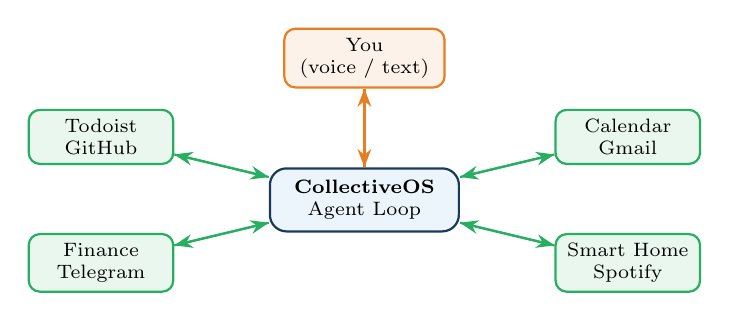
\begin{tikzpicture}[node distance=0.7cm, every node/.style={font=\scriptsize}]
  % Center
  \node[draw=primary, fill=lightblue, rounded corners=6pt, thick,
        minimum width=2.4cm, minimum height=0.8cm, align=center]
        (core) {\textbf{CollectiveOS}\\Agent Loop};

  % User
  \node[obox=1.8cm, above=1.0cm of core] (user) {You\\(voice / text)};

  % Connectors arranged around
  \node[gbox=1.6cm, right=1.2cm of core, yshift= 0.8cm] (cal)  {Calendar\\Gmail};
  \node[gbox=1.6cm, right=1.2cm of core, yshift=-0.8cm] (dev)  {Smart Home\\Spotify};
  \node[gbox=1.6cm, left=1.2cm of core,  yshift= 0.8cm] (task) {Todoist\\GitHub};
  \node[gbox=1.6cm, left=1.2cm of core,  yshift=-0.8cm] (fin)  {Finance\\Telegram};

  % Arrows
  \draw[-{Stealth}, thick, colorange] (user) -- (core);
  \draw[-{Stealth}, thick, colorange] (core) -- (user);
  \draw[-{Stealth}, thick, colgreen]  (core) -- (cal);
  \draw[-{Stealth}, thick, colgreen]  (cal)  -- (core);
  \draw[-{Stealth}, thick, colgreen]  (core) -- (dev);
  \draw[-{Stealth}, thick, colgreen]  (dev)  -- (core);
  \draw[-{Stealth}, thick, colgreen]  (core) -- (task);
  \draw[-{Stealth}, thick, colgreen]  (task) -- (core);
  \draw[-{Stealth}, thick, colgreen]  (core) -- (fin);
  \draw[-{Stealth}, thick, colgreen]  (fin)  -- (core);
\end{tikzpicture}
\end{center}
\end{column}
\end{columns}
\end{frame}

% ── 2. Problem / Use Case ─────────────────────────────────────────────────────
\begin{frame}{Problem / Use Case}
\begin{columns}[T]
\begin{column}{0.31\textwidth}
\begin{alertblock}{Today}
\scriptsize
\textbf{Fragmented workflows:}
\begin{itemize}
  \item Open Calendar app to check schedule
  \item Open Gmail for emails
  \item Switch to Spotify to change music
  \item Open Todoist for tasks
  \item Manually copy context between apps
  \item No memory across sessions
  \item 10+ context switches per hour
\end{itemize}
\end{alertblock}
\end{column}
\begin{column}{0.03\textwidth}
\begin{center}\vspace{2em}{\Large\color{accent}$\rightarrow$}\end{center}
\end{column}
\begin{column}{0.31\textwidth}
\begin{block}{With CollectiveOS}
\scriptsize
\textbf{One conversation:}
\begin{itemize}
  \item ``What's on my calendar?''
  \item ``Any urgent emails?''
  \item ``Play focus music''
  \item ``Add task: review PR''
  \item Shared context, one interface
  \item Remembers past conversations
  \item Zero context switching
\end{itemize}
\end{block}
\end{column}
\begin{column}{0.03\textwidth}
\begin{center}\vspace{2em}{\Large\color{colgreen}$\rightarrow$}\end{center}
\end{column}
\begin{column}{0.27\textwidth}
\begin{exampleblock}{Real Example}
\scriptsize
\textbf{User (voice):}\\
``Hey Collective, clear my morning \& reschedule the 10am standup to 2pm''

\vspace{0.5em}
\textbf{CollectiveOS:}\\
→ Reads calendar\\
→ Asks confirmation\\
→ Moves event\\
→ Confirms back

\vspace{0.5em}
\textbf{One utterance.\\Zero app switches.}
\end{exampleblock}
\end{column}
\end{columns}
\end{frame}

% ── 3. Current Capabilities ───────────────────────────────────────────────────
\begin{frame}{Current Capabilities}
\begin{columns}[T]
\begin{column}{0.48\textwidth}
\begin{block}{Working Now}
\scriptsize
\begin{tabular}{p{0.3cm}p{4.5cm}}
\done & Gemini Flash agent loop (function calling) \\
\done & Intent router — narrows 57 tools per message \\
\done & 25+ connector stubs (Calendar, Gmail, Todoist, Spotify, GitHub, Home Assistant, Finance, \ldots) \\
\done & Semantic memory — embed + pgvector retrieval \\
\done & Knowledge graph — entity extraction, GraphRAG \\
\done & Permission system — connector toggle + write gate \\
\done & FastAPI with SSE streaming (\ic{/chat/stream}) \\
\done & Scheduled routines — APScheduler + cron \\
\done & Telegram integration (fire-and-forget webhook) \\
\done & AI model comparison (\ic{ai\_compare}) \\
\done & Full observability — token cost, tool latency, structlog \\
\done & Voice mode — VoiceOS integration (LiveKit + Gemini Live) \\
\done & Wake word gate — ``hey collective'' activates voice \\
\done & Bilingual (Hindi + English) voice responses \\
\done & Write-action confirmation gate in voice pipeline \\
\end{tabular}
\end{block}
\end{column}
\begin{column}{0.48\textwidth}
\begin{alertblock}{Partial / In Progress}
\scriptsize
\begin{tabular}{p{0.3cm}p{4.5cm}}
{\color{colorange}$\sim$} & PostgreSQL not auto-started — memory silently skips when DB is offline \\
{\color{colorange}$\sim$} & \ic{DISABLE\_EMBEDDINGS=1} workaround active — sentence-transformers bypassed to avoid asyncio deadlock \\
{\color{colorange}$\sim$} & Connectors mostly stubbed — Calendar/Gmail need OAuth token flow \\
{\color{colorange}$\sim$} & Voice sessions require manual VoiceOS startup \\
{\color{colorange}$\sim$} & Single-user only — no multi-tenant auth \\
\end{tabular}
\end{alertblock}
\vspace{0.4em}
\begin{exampleblock}{Architecture Constraint}
\scriptsize
\textbf{Read-only first.} Every connector is built read-only first.
Write actions require an \textbf{explicit confirmation step} — enforced
at the code level (not just in the system prompt).
\end{exampleblock}
\end{column}
\end{columns}
\end{frame}

% ── 4. System Architecture ────────────────────────────────────────────────────
\begin{frame}{System Architecture — Augmented LLM Pattern}
\begin{center}
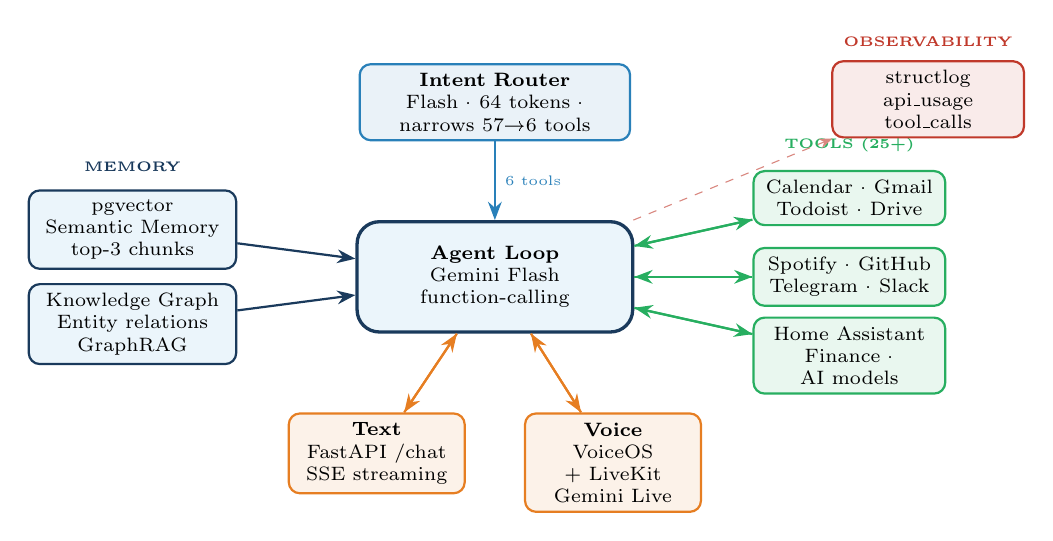
\begin{tikzpicture}[node distance=0.6cm and 0.5cm,
                    every node/.style={font=\scriptsize}]

  % === Central Agent Loop ===
  \node[draw=primary, fill=lightblue, rounded corners=8pt, very thick,
        minimum width=3.5cm, minimum height=1.4cm, align=center]
        (loop) {\textbf{Agent Loop}\\Gemini Flash\\function-calling};

  % === Router (top) ===
  \node[abox=3.2cm, above=1.0cm of loop] (router)
        {\textbf{Intent Router}\\Flash · 64 tokens · narrows 57→6 tools};
  \draw[-{Stealth}, thick, accent] (router) -- node[right]{\tiny 6 tools} (loop);

  % === Memory (left) ===
  \node[pbox=2.4cm, left=1.5cm of loop, yshift=0.6cm] (vec)
        {pgvector\\Semantic Memory\\top-3 chunks};
  \node[pbox=2.4cm, left=1.5cm of loop, yshift=-0.6cm] (graph)
        {Knowledge Graph\\Entity relations\\GraphRAG};
  \draw[-{Stealth}, thick, primary] (vec)   -- (loop);
  \draw[-{Stealth}, thick, primary] (graph) -- (loop);
  \node[above=0.1cm of vec, font=\tiny\bfseries, text=primary] {MEMORY};

  % === Tools (right) ===
  \node[gbox=2.2cm, right=1.5cm of loop, yshift= 1.0cm] (t1)
        {Calendar · Gmail\\Todoist · Drive};
  \node[gbox=2.2cm, right=1.5cm of loop, yshift= 0.0cm] (t2)
        {Spotify · GitHub\\Telegram · Slack};
  \node[gbox=2.2cm, right=1.5cm of loop, yshift=-1.0cm] (t3)
        {Home Assistant\\Finance · AI models};
  \draw[-{Stealth}, thick, colgreen] (loop) -- (t1);
  \draw[-{Stealth}, thick, colgreen] (t1)   -- (loop);
  \draw[-{Stealth}, thick, colgreen] (loop) -- (t2);
  \draw[-{Stealth}, thick, colgreen] (t2)   -- (loop);
  \draw[-{Stealth}, thick, colgreen] (loop) -- (t3);
  \draw[-{Stealth}, thick, colgreen] (t3)   -- (loop);
  \node[above=0.1cm of t1, font=\tiny\bfseries, text=colgreen] {TOOLS (25+)};

  % === User / Voice (bottom) ===
  \node[obox=2.0cm, below=1.0cm of loop, xshift=-1.5cm] (text)
        {\textbf{Text}\\FastAPI /chat\\SSE streaming};
  \node[obox=2.0cm, below=1.0cm of loop, xshift= 1.5cm] (voice)
        {\textbf{Voice}\\VoiceOS + LiveKit\\Gemini Live};
  \draw[-{Stealth}, thick, colorange] (text)  -- (loop);
  \draw[-{Stealth}, thick, colorange] (loop)  -- (text);
  \draw[-{Stealth}, thick, colorange] (voice) -- (loop);
  \draw[-{Stealth}, thick, colorange] (loop)  -- (voice);

  % === Observability (top right corner) ===
  \node[rbox=2.2cm, above=0.4cm of t1, xshift=1.0cm] (obs)
        {structlog\\api\_usage\\tool\_calls};
  \draw[-{Stealth}, dashed, colred!60] (loop) -- (obs);
  \node[above=0.05cm of obs, font=\tiny\bfseries, text=colred] {OBSERVABILITY};

\end{tikzpicture}
\end{center}
\end{frame}

% ── 5. End-to-End Workflow (animated) ─────────────────────────────────────────
\begin{frame}{End-to-End Workflow}
\begin{center}
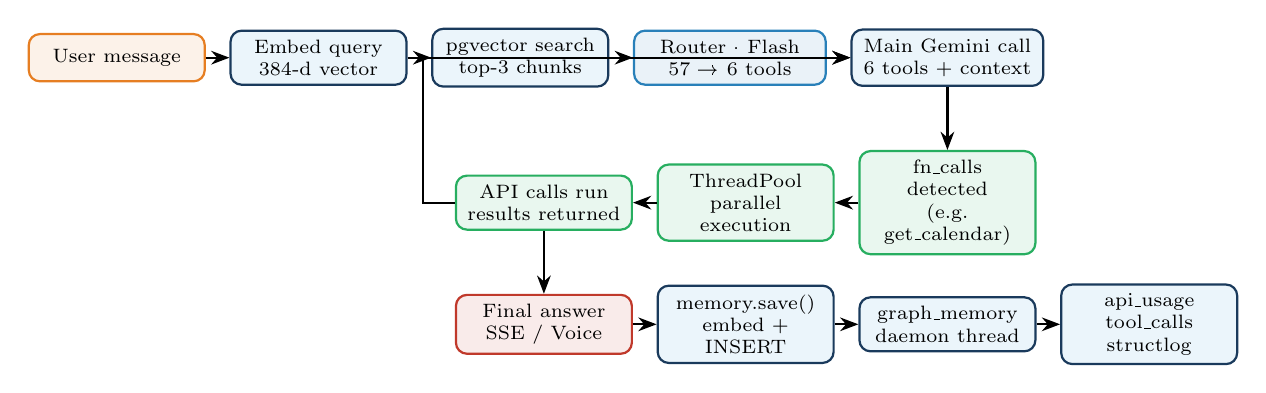
\begin{tikzpicture}[node distance=0.4cm and 0.35cm,
                    every node/.style={font=\tiny}]

  % Row 1 — Ingestion ──────────────────────────────────────────────────────────
  \node[obox=2.0cm] (user) {User message};

  \visible<2->{
    \node[pbox=2.0cm, right=0.3cm of user] (embed) {Embed query\\384-d vector};
    \node[pbox=2.0cm, right=0.3cm of embed] (mem)  {pgvector search\\top-3 chunks};
    \draw[-{Stealth},thick] (user)  -- (embed);
    \draw[-{Stealth},thick] (embed) -- (mem);
  }

  \visible<3->{
    \node[abox=2.2cm, right=0.3cm of mem] (router) {Router · Flash\\57 → 6 tools};
    \node[pbox=2.2cm, right=0.3cm of router] (main) {Main Gemini call\\6 tools + context};
    \draw[-{Stealth},thick] (mem)    -- (router);
    \draw[-{Stealth},thick] (router) -- (main);
  }

  % Row 2 — Execution ──────────────────────────────────────────────────────────
  \visible<4->{
    \node[gbox=2.0cm, below=0.8cm of main] (fn)  {fn\_calls detected\\(e.g.\ get\_calendar)};
    \node[gbox=2.0cm, left=0.3cm of fn]   (par) {ThreadPool\\parallel execution};
    \node[gbox=2.0cm, left=0.3cm of par]  (api) {API calls run\\results returned};
    \draw[-{Stealth},thick] (main) -- (fn);
    \draw[-{Stealth},thick] (fn)   -- (par);
    \draw[-{Stealth},thick] (par)  -- (api);
    \draw[-{Stealth},thick] (api.west) -- ++(-0.4,0) |- (main.west);
  }

  % Row 3 — Response + Post-processing ─────────────────────────────────────────
  \visible<5->{
    \node[rbox=2.0cm, below=0.8cm of api] (out)  {Final answer\\SSE / Voice};
    \node[pbox=2.0cm, right=0.3cm of out] (save) {memory.save()\\embed + INSERT};
    \node[pbox=2.0cm, right=0.3cm of save] (gm)  {graph\_memory\\daemon thread};
    \node[pbox=2.0cm, right=0.3cm of gm]  (obs)  {api\_usage\\tool\_calls\\structlog};
    \draw[-{Stealth},thick] (api)  -- (out);
    \draw[-{Stealth},thick] (out)  -- (save);
    \draw[-{Stealth},thick] (save) -- (gm);
    \draw[-{Stealth},thick] (gm)   -- (obs);
  }

\end{tikzpicture}
\end{center}

\vspace{0.2em}
\begin{columns}
\begin{column}{0.25\textwidth}
\visible<2->{\begin{block}{\centering Step 1}\centering\scriptsize Embed + retrieve memory context\end{block}}
\end{column}
\begin{column}{0.25\textwidth}
\visible<3->{\begin{block}{\centering Step 2}\centering\scriptsize Router narrows tools, Gemini reasons\end{block}}
\end{column}
\begin{column}{0.25\textwidth}
\visible<4->{\begin{block}{\centering Step 3}\centering\scriptsize Tools run in parallel, loop repeats\end{block}}
\end{column}
\begin{column}{0.25\textwidth}
\visible<5->{\begin{exampleblock}{\centering Step 4}\centering\scriptsize Stream reply, save memory, log cost\end{exampleblock}}
\end{column}
\end{columns}
\end{frame}

% ── 6. Live Demo ──────────────────────────────────────────────────────────────
\begin{frame}{Live Demo}
\begin{columns}[T]
\begin{column}{0.48\textwidth}
\begin{block}{Demo Script}
\begin{enumerate}\scriptsize
  \item \textbf{Start both services}
  \begin{itemize}
    \item CollectiveOS: \ic{DISABLE\_EMBEDDINGS=1 collectiveos voice --port 8000}
    \item VoiceOS: \ic{.venv/bin/voice-service console}
  \end{itemize}
  \item \textbf{Wake the assistant}\\
    Say: \textit{``Hey Collective''}\\
    → Agent activates. No action taken before wake word.
  \item \textbf{Simple lookup (English)}\\
    Say: \textit{``What time is it?''}\\
    → Answers locally in English.
  \item \textbf{Simple lookup (Hindi)}\\
    Say: \textit{``Aaj mera schedule kya hai?''}\\
    → Responds in Hindi.
  \item \textbf{Write action (confirmation gate)}\\
    Say: \textit{``Add a task: review the PR''}\\
    → Describes action, waits for ``yes'' before executing.
\end{enumerate}
\end{block}
\end{column}
\begin{column}{0.48\textwidth}
\begin{alertblock}{What to Observe}
\scriptsize
\begin{itemize}
  \item Wake word gate: speech before ``hey collective'' is ignored
  \item Language matching: reply language mirrors what the user spoke
  \item Step-by-step confirmation: write actions never proceed without approval
  \item Structured logs appear in terminal with token counts and cost per call
\end{itemize}
\end{alertblock}
\vspace{0.4em}
\begin{exampleblock}{What the Logs Show (terminal)}
\scriptsize
\begin{verbatim}
WebSocket /v1/ws [accepted]
api_call model=gemini-flash-lite
  input_tokens=1223 output_tokens=3
  cost_usd=0.000124 source=router
api_call model=gemini-flash-lite
  input_tokens=908 output_tokens=27
  cost_usd=0.000102 source=chat
\end{verbatim}
\end{exampleblock}
\end{column}
\end{columns}
\end{frame}

% ── 7. Current Limitations ────────────────────────────────────────────────────
\begin{frame}{Current Limitations}
\begin{center}
\scriptsize
\begin{tabular}{p{3.8cm}p{4.2cm}p{4.5cm}}
\toprule
\textbf{Limitation} & \textbf{Root Cause} & \textbf{Fix / Path Forward} \\
\midrule
PostgreSQL not auto-started; memory retrieval silently skipped &
DB not managed by the app; requires manual \ic{pg\_ctl start} &
Add \ic{docker-compose.yml} or launchd plist; health-check at startup \\[0.4em]

\ic{DISABLE\_EMBEDDINGS=1} active; no vector search &
PyTorch/gRPC mutex deadlock with uvicorn's asyncio event loop &
Isolate embedding model in a subprocess or side-car; pass results over a queue \\[0.4em]

Connectors are mostly stubbed; no live API data &
OAuth flows not yet wired &
Phase 3: add OAuth token fetch, store encrypted in \ic{credentials} table \\[0.4em]

Voice requires manual VoiceOS startup &
VoiceOS is a separate service (LiveKit-based) &
Add a process manager (Supervisor / Docker Compose) to boot both together \\[0.4em]

Single-user only &
Auth is a single API token from \ic{.env} &
Phase 5: FastAPI JWT auth; per-user \ic{credentials} row \\[0.4em]

Write confirmation is voice-only &
\ic{confirm\_fn} wired only in \ic{voice\_gateway.py} &
Add confirmation to text \ic{/chat} endpoint with SSE event type \\
\bottomrule
\end{tabular}
\end{center}
\end{frame}

% ── 8. Next Milestones ────────────────────────────────────────────────────────
\begin{frame}{Next Milestones}
\begin{columns}[T]
\begin{column}{0.48\textwidth}
\begin{block}{Near Term}
\scriptsize
\begin{tabular}{p{0.3cm}p{5.0cm}}
{\color{colorange}1} & Auto-start PostgreSQL; re-enable embeddings and vector memory \\[0.2em]
{\color{colorange}2} & Wire first real OAuth flow — Google Calendar read + confirmed write \\[0.2em]
{\color{colorange}3} & Gmail read (recent inbox) + draft reply with confirmation \\[0.2em]
{\color{colorange}4} & End-to-end smoke test: morning briefing routine via Telegram \\[0.2em]
{\color{colorange}5} & Fix embedding isolation — move model to subprocess \\
\end{tabular}
\end{block}
\vspace{0.3em}
\begin{block}{Medium Term}
\scriptsize
\begin{tabular}{p{0.3cm}p{5.0cm}}
{\color{accent}6} & Google Drive read; Todoist full sync \\[0.2em]
{\color{accent}7} & Home Assistant — full device state + switch control \\[0.2em]
{\color{accent}8} & Web chat UI (plain HTML + JS served by FastAPI) \\
\end{tabular}
\end{block}
\end{column}
\begin{column}{0.48\textwidth}
\begin{block}{Roadmap (from \ic{docs/mvp\_plan.md})}
\scriptsize
\begin{tabular}{lll}
\toprule
\textbf{Phase} & \textbf{Goal} & \textbf{Status} \\
\midrule
0 & Skeleton / agent loop & \textcolor{colgreen}{Done} \\
1 & First real connector   & \textcolor{colgreen}{Done} \\
2 & Postgres-backed memory & \textcolor{colorange}{Partial} \\
3 & Services (Cal, Gmail, Drive) & \textcolor{colorange}{Partial} \\
4 & Devices (Home Assistant) & \textcolor{colorange}{Partial} \\
5 & FastAPI layer          & \textcolor{colgreen}{Done} \\
6 & Voice interface        & \textcolor{colgreen}{Done} \\
\bottomrule
\end{tabular}
\end{block}
\vspace{0.3em}
\begin{alertblock}{Principle}
\scriptsize
\textbf{One domain end-to-end before the next.}
Get Calendar read + write fully working with real data before adding Gmail.
\end{alertblock}
\end{column}
\end{columns}
\end{frame}

% =============================================================================
\section{Technical Demo / Walkthrough}
% =============================================================================

\begin{frame}{One Complete Journey — Input to Logs}
\begin{center}
\textit{\small ``Hey Collective, reschedule my 10am standup to 2pm''}
\end{center}

\vspace{0.3em}

\begin{center}
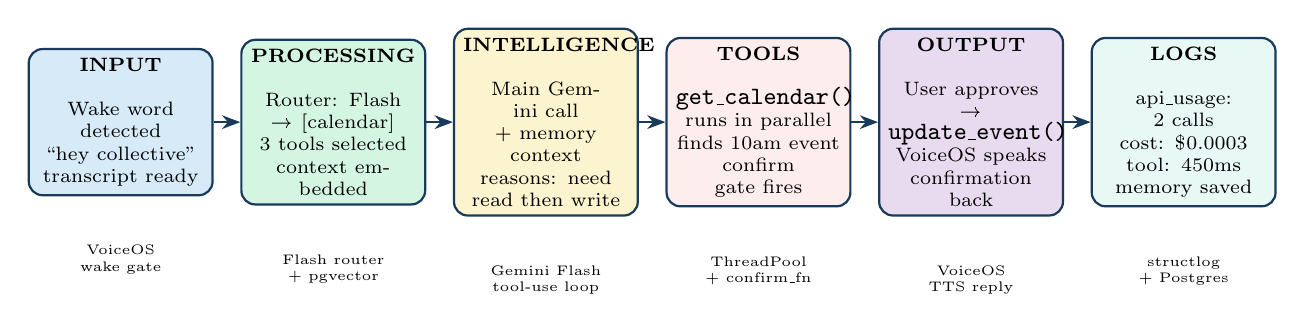
\begin{tikzpicture}[node distance=0.55cm, every node/.style={font=\tiny}]

  % Stage nodes (horizontal)
  \node[stagebox=stagecol1] (s1) at (0,0)    {\textbf{INPUT}\\~\\Wake word\\detected\\``hey collective''\\transcript ready};

  \visible<2->{
  \node[stagebox=stagecol2] (s2) at (2.7,0)  {\textbf{PROCESSING}\\~\\Router: Flash\\→ [calendar]\\3 tools selected\\context embedded};
  \draw[-{Stealth},thick,primary] (s1) -- (s2);
  }

  \visible<3->{
  \node[stagebox=stagecol3] (s3) at (5.4,0)  {\textbf{INTELLIGENCE}\\~\\Main Gemini call\\+\ memory context\\reasons: need\\read then write};
  \draw[-{Stealth},thick,primary] (s2) -- (s3);
  }

  \visible<4->{
  \node[stagebox=stagecol4] (s4) at (8.1,0)  {\textbf{TOOLS}\\~\\\ic{get\_calendar()}\\runs in parallel\\finds 10am event\\confirm gate fires};
  \draw[-{Stealth},thick,primary] (s3) -- (s4);
  }

  \visible<5->{
  \node[stagebox=stagecol5] (s5) at (10.8,0) {\textbf{OUTPUT}\\~\\User approves\\→ \ic{update\_event()}\\VoiceOS speaks\\confirmation back};
  \draw[-{Stealth},thick,primary] (s4) -- (s5);
  }

  \visible<6->{
  \node[stagebox=stagecol6] (s6) at (13.5,0) {\textbf{LOGS}\\~\\api\_usage: 2 calls\\cost: \$0.0003\\tool: 450ms\\memory saved};
  \draw[-{Stealth},thick,primary] (s5) -- (s6);
  }

  % Step labels below
  \node[below=0.5cm of s1, text width=2.1cm, align=center] {VoiceOS\\wake gate};
  \visible<2->{\node[below=0.5cm of s2, text width=2.1cm, align=center] {Flash router\\+ pgvector};}
  \visible<3->{\node[below=0.5cm of s3, text width=2.1cm, align=center] {Gemini Flash\\tool-use loop};}
  \visible<4->{\node[below=0.5cm of s4, text width=2.1cm, align=center] {ThreadPool\\+ confirm\_fn};}
  \visible<5->{\node[below=0.5cm of s5, text width=2.1cm, align=center] {VoiceOS\\TTS reply};}
  \visible<6->{\node[below=0.5cm of s6, text width=2.1cm, align=center] {structlog\\+ Postgres};}

\end{tikzpicture}
\end{center}

\vspace{0.2em}
\begin{columns}
\begin{column}{0.16\textwidth}
\visible<1->{\begin{exampleblock}{\centering Input}
\centering\scriptsize Wake word\\+ transcript\\extracted
\end{exampleblock}}
\end{column}
\begin{column}{0.16\textwidth}
\visible<2->{\begin{block}{\centering Processing}
\centering\scriptsize Router cuts\\token cost\\8$\times$
\end{block}}
\end{column}
\begin{column}{0.16\textwidth}
\visible<3->{\begin{block}{\centering Logic}
\centering\scriptsize Model decides\\read first,\\write second
\end{block}}
\end{column}
\begin{column}{0.16\textwidth}
\visible<4->{\begin{alertblock}{\centering Tools}
\centering\scriptsize Read runs free;\\ write is\\gated
\end{alertblock}}
\end{column}
\begin{column}{0.16\textwidth}
\visible<5->{\begin{block}{\centering Output}
\centering\scriptsize Bilingual,\\step-by-step,\\voice only
\end{block}}
\end{column}
\begin{column}{0.16\textwidth}
\visible<6->{\begin{exampleblock}{\centering Logs}
\centering\scriptsize Every call\\tracked,\\cost visible
\end{exampleblock}}
\end{column}
\end{columns}
\end{frame}

% =============================================================================
\section{Engineering Status / Build Report}
% =============================================================================

\begin{frame}{Engineering Status / Build Report}
\begin{columns}[T]
\begin{column}{0.50\textwidth}
\begin{block}{Phase Completion}
\scriptsize
\begin{tabular}{p{0.3cm}lp{3.5cm}}
\toprule
 & \textbf{Phase} & \textbf{Key Deliverable} \\
\midrule
\done & Phase 0 — Skeleton & Agent loop + placeholder tools \\
\done & Phase 1 — Real connectors & 25+ connector definitions \\
{\color{colorange}$\sim$} & Phase 2 — Postgres memory & Schema done; DB not auto-started \\
{\color{colorange}$\sim$} & Phase 3 — Services & Connectors stubbed; OAuth pending \\
{\color{colorange}$\sim$} & Phase 4 — Devices & Home Assistant partial \\
\done & Phase 5 — FastAPI layer & \ic{/chat}, \ic{/chat/stream}, \ic{/voice/ws} \\
\done & Phase 6 — Voice & VoiceOS + wake word + bilingual \\
\bottomrule
\end{tabular}
\end{block}
\vspace{0.3em}
\begin{block}{Recent Major Changes (this sprint)}
\scriptsize
\begin{itemize}
  \item Migrated LLM backend: Anthropic SDK → Gemini (\ic{google-genai})
  \item Added \ic{collectiveos voice} CLI command
  \item Fixed voice contract event shapes (pydantic validation)
  \item Added \ic{confirm\_fn} hard gate for write tools in voice pipeline
  \item VoiceOS PR\#8 merged: \ic{WakeState} + \ic{\_PendingAction} confirmation gate
\end{itemize}
\end{block}
\end{column}
\begin{column}{0.46\textwidth}
\begin{exampleblock}{Live Metrics (sampled from logs)}
\scriptsize
\begin{tabular}{ll}
\toprule
\textbf{Metric} & \textbf{Value} \\
\midrule
Model (main)        & \ic{gemini-flash-lite-latest} \\
Router cost/call    & $\approx\$0.000124$ (1{,}223 in / 3 out) \\
Chat cost/call      & $\approx\$0.000102$ (908 in / 27 out) \\
Total (typical msg) & $\approx\$0.00025$ \\
First token         & $\approx 1.2$s \\
Full response       & $\approx 3$s \\
Tool (web\_search)  & $\approx 842$ms avg \\
\bottomrule
\end{tabular}
\end{exampleblock}
\vspace{0.3em}
\begin{alertblock}{Blockers}
\scriptsize
\begin{enumerate}
  \item \textbf{Postgres not running} — memory \& observability writes skip silently
  \item \textbf{Embedding isolation} — PyTorch mutex deadlocks uvicorn event loop; \ic{DISABLE\_EMBEDDINGS=1} active
  \item \textbf{OAuth not wired} — connectors return stub data
\end{enumerate}
\end{alertblock}
\begin{block}{Branch}
\scriptsize
\ic{feature/gemini-backend} — PR ready:\\
\ic{github.com/Anurag9Dhiman/CollectiveOS}
\end{block}
\end{column}
\end{columns}
\end{frame}

% ─── Thank-you slide ─────────────────────────────────────────────────────────
\begin{frame}[c]
\begin{center}
{\Huge\color{primary}\textbf{Thank You}}\\[1em]
{\large Questions?}\\[2em]
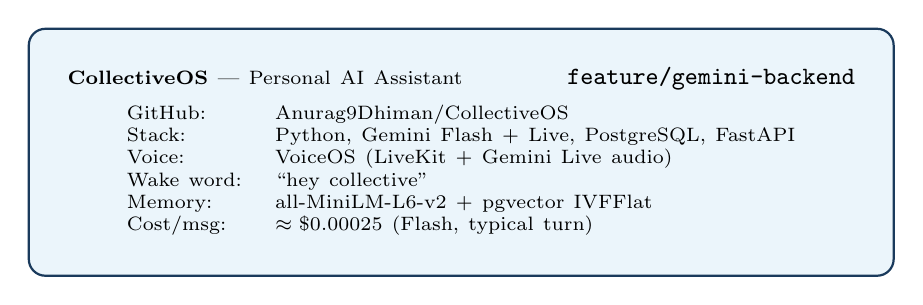
\begin{tikzpicture}
  \node[draw=primary, fill=lightblue, rounded corners=6pt, thick,
        inner sep=14pt, text width=10cm, align=center] {
    \scriptsize
    \textbf{CollectiveOS} --- Personal AI Assistant \hfill \ic{feature/gemini-backend}\\[0.5em]
    \begin{tabular}{ll}
      GitHub:     & Anurag9Dhiman/CollectiveOS \\
      Stack:      & Python, Gemini Flash + Live, PostgreSQL, FastAPI \\
      Voice:      & VoiceOS (LiveKit + Gemini Live audio) \\
      Wake word:  & ``hey collective'' \\
      Memory:     & all-MiniLM-L6-v2 + pgvector IVFFlat \\
      Cost/msg:   & $\approx\$0.00025$ (Flash, typical turn) \\
    \end{tabular}
  };
\end{tikzpicture}
\end{center}
\end{frame}

\end{document}
